\chapter{The role of TNF-alpha in tinnitus}

\section{Overview}

\newrefsection

\section{Introduction}
Tinnitus is the perception of sound in the absence of acoustic stimuli. The potential causes of tinnitus are diverse, but the biggest risk factor is hearing loss. Previous research has indicated that hearing loss activates neural plasticity mechanisms in the central auditory pathway, which is widely believed to contribute to tinnitus (\cite{Roberts2010}). Of particular interest is homeostatic plasticity---the capacity of a neuron to adjust its synaptic transmission and intrinsic membrane properties to maintain its overall level of activity (\cite{Turrigiano1999, Davis2001}). For example, when sensory input is weakened by hearing loss, neurons in the auditory pathway become more excitable by adjusting their synaptic strengths and intrinsic membrane properties through homeostatic plasticity (\cite{Kotak2005, Yang2011a, Yang2012}). Following noise-induced hearing lesion, the expression of glutamic acid decarboxylase (GAD), the enzyme that synthesizes inhibitory neural transmitter GABA, is down-regulated in the dorsal cochlear nucleus, inferior colliculus, and auditory cortex (\cite{Abbott1999, Milbrandt2000, Yang2011a, Browne2012}). Consequently, noise-induced hearing lesion results in reduced GABA release, reduced tonic inhibition and enhanced excitability in cortical pyramidal neurons (\cite{Yang2011a, Yang2012}). Down-regulation of GABAergic inhibition is considered a potential mechanism for tinnitus (\cite{Yang2011a, Llano2012}).

Tumor necrosis factor-\textalpha{} (TNF-\textalpha{}) is a pro-inflammatory cytokine that also plays an important role in homeostatic plasticity in the central nervous system (\cite{Stellwagen2005, Stellwagen2006, Steinmetz2010, Wang2011}). For example, TNF-\textalpha{} sequestration with a soluble form of TNF receptor blocks TTX treatment-induced up-scaling of glutamate synapses in cultured neurons (\cite{Stellwagen2006, Steinmetz2010}). Relevant to reduced neuronal inhibition as a potential tinnitus mechanism, TNF-\textalpha{} mediates TTX-induced down-regulation of GABAergic activity \textit{in vitro} by regulating endocytosis of GABA$_\mathrm{A}$ receptors (\cite{Stellwagen2005, Stellwagen2006}).

TNF-\textalpha{} is also involved in homeostatic modulation of central auditory neurons. Although TNF-\textalpha{} knockout mice have normal gross brain structure, Hebbian LTP (\cite{Kaneko2008}) and tone-induced map reorganization (\cite{Yang2013}) compared to wildtype controls, TNF-\textalpha{} knockout mice showed weaker cortical response to tones, suggesting that while wildtype mice can up-regulate cortical responses in the relatively impoverished acoustic environment of the vivarium, the knockout mice lacked such homeostatic plasticity (\cite{Yang2013}). When acoustically over stimulated, wildtype mice showed homeostatic down regulation of cortical responses to sounds, while TNF-\textalpha{} knockout mice showed enhanced responses (\cite{Yang2013}), indicative of a lack of homeostatic regulation of cortical responses by the level of sensory input.

In the present study we examined the role of TNF-\textalpha{} in noise-induced tinnitus. We found that monaural hearing loss-induced aural dominance shift was largely absent in the KO mice. Wildtype but not TNF-\textalpha{} knockout mice developed tinnitus after monaural noise exposure. Infusion of recombinant mouse TNF-\textalpha{} protein into the auditory cortex resulted in tinnitus in both wildtype and TNF-\textalpha{} knockout mice without noise exposure.

\section{Methods}

\subsection{Noise exposure and auditory brainstem response (ABR)}
All experimental procedures were reviewed and approved by UC Berkeley Animal Care and Use Committee. TNF-\textalpha{} KO mice and corresponding C57BL/6 WT mice were originally purchased from the Jackson Laboratory, and were bred in a UC Berkeley animal facility. Animals were anesthetized with ketamine (100 mg/kg, IP) and xylazine (10 mg/kg, IP), and maintained at 36.5$^\circ$C with a homeothermic heating pad (Harvard Apparatus). Unilateral noise-induced hearing loss (NIHL) was performed in a sound attenuation chamber by playing a continuous pure tone of 8 kHz at 112 dB SPL through a calibrated custom-made piezo earphone speaker to the left ear of the mouse for 2 hours, while the right ear was protected with sound attenuating clay. The sound level was calibrated with a Br\"uel and Kj\ae r 4135 condenser microphone (N\ae rum, Denmark) before and after the NIHL.

Hearing thresholds were assessed using auditory brainstem responses (ABR). ABR signals were recorded using the BioSigRP software on a TDT RX5 Sys3 recording device. Tone pips (3-ms full-cycle sine waves at 4, 8, 16 and 32 kHz at 5-dB intensity steps from 0 to 70 dB SPL) were delivered to the ears at a rate of 19 times per second through a calibrated TDT earphone, and 500 recordings were averaged to generate each ABR trace. ABR signals were recorded with three electrodes subcutaneously inserted behind the ear ipsilateral to the speaker, at the vertex of the head, and at the back of the body near the tail. The sound level that activated a minimal discernable response was defined as the auditory threshold for the particular frequency for each ear.

\subsection{Behavioral test of tinnitus with a gap detection task}
Tinnitus was assessed using the gap detection paradigm (\cite{Turner2006}). The gap detection task measures the acoustic startle response elicited by a brief white noise pulse and its suppression by a preceding silent gap embedded in a background sound. This paradigm has recently been confirmed to detect tinnitus in human subjects (\cite{Fournier2013}). Mice were placed in a small box, which rested atop a piezoelectric sensor within a sound attenuation chamber. Sounds were played through an open field speaker (FOSTEX FT17H) fixed above the small box. Each trial began with a carrier pure tone (frequency pseudorandomly selected from 5, 7, 10, 14, 20, 28, or 45 kHz, all at 75 dB SPL), played for 10-20 s. In uncued trials, the carrier tone was followed by a startle stimulus---a 50 ms white noise burst at 102 dB SPL. In cued trials, the startle stimulus was preceded by 50 ms of silence 100 ms prior to its onset. In each testing session, the animal performed a total of 500 trials (50\% cued and 50\% uncued). After each session, we calculated the startle response ratio, which is defined as the average startle amplitude to the cued trials divided by the average amplitude of the uncued trials. The startle response ratio signifies a silent-gap induced reduction of the startle response. For example, a startle response ratio of 0.6 indicates a 40\% reduction of the startle amplitude for the cued trials. A startle response ratio of 1 suggests that the animal failed to detect the silent gap.

To assess an animal's ability to perform an auditory task, distinct from its ability to detect a silent gap, the pre-pulse inhibition (PPI) task was administered in a separate group of mice immediately before and after (2 d and 10 d) NIHL. The physical setup for the PPI task was identical to that for gap detection. However, the trial structure differed in that carrier tone was absent and a white noise burst was cued by a 50-ms pure tone pulse (frequency pseudorandomly selected from 5, 7, 10, 14, 20, 28, or 45 kHz, all at 75 dB SPL). In short, the PPI task tests an animal's ability to detect a pure tone pulse in silence, while the gap detection task measures an animal's ability to detect a silent gap in a continuous pure tone.

Mice were first acclimated to the testing chamber and trained until the behavior stabilized across two days. On average, 1000 trials were given prior to the first test session. We compared individual animals' performance before and after the experimental manipulation. An increase of gap ratio accompanied by i) normal ABR for the intact ear and ii) normal PPI behavior were assumed to indicate tinnitus. Because both the gap detection task and the PPI task require normal hearing and hearing sensitivity above 32 kHz was highly variable across animals, only trials with carrier frequencies between 5 and 20 kHz were included in the final analysis.

\subsection{Injection of recombinant TNF-\textalpha{} in the auditory cortex}
Mice were anaesthetized with ketamine (100 mg/kg, IP) and xylazine (10 mg/kg, IP). Injection was done stereotactically to the right auditory cortex. A burr hole was made on the temporal ridge 1.75 mm anterior to the transverse suture. A pulled glass micropipette filled with recombinant mouse TNF-\textalpha{} (66.6 ng/\textmu l in 1\% mouse albumin fraction V) or 1\% mouse albumin fraction V solution was lowered to 500 \textmu m below the pial surface and 1.5 \textmu l solution was injected at 100 nl/min by pressure injection (Stoelting Quintessential Injector, Wood Dale, IL, USA). The micropipette was then retracted 250 \textmu m and an additional 1.5 \textmu l of virus solution was injected. To minimize leaking, the micropipette was left in place for 8 min after each injection. In total, the experimental group received a dose of 200 ng of recombinant TNF-\textalpha{} to right auditory cortex. After injection, the skin was sutured and the animals were returned to their home cages after regaining movement. For postoperative pain management, animals received subcutaneous injection of buprenorphine (0.05 mg/kg, SQ) and meloxicam (2 mg/kg, SQ).

\subsection{Measuring GAD65 mRNA levels with RT-PCR}
After behavioral testing, animals were euthanized with isoflurane. Brain tissue was collected from the right and left auditory cortices based on anatomical landmarks by an experienced experimenter. A coronal slice of approximately 1 mm thickness (estimated stereotaxic coordinates: -2 mm to -3 mm bregma) was made using the dorsal-ventral extent of the hippocampus as landmarks. We then hemisected and isolated the auditory cortex at each side by making two orthogonal cuts to the cortical surface at 1 mm and 2 mm dorsal to the lingual gyrus. Subcortical structures were removed and two 1-mm cubes of cortical tissue, one from each side, were collected. These samples presumably included the primary auditory cortex and possibly other fields of the auditory cortex.

Reverse transcription polymerase chain reaction (RT-PCR) was conducted by an experimenter who was blind to the experimental conditions. Total RNA samples were prepared from the tissue with RNA Wiz (Ambion) according to the manufacturer's instructions. The total RNA obtained ($\sim$3 \textmu g) was reverse-transcribed using a first-strand cDNA synthesis kit (BD Biosciences, Palo Alto, CA). The PCR mixture (50 \textmu l) contained 10$\times$ Taq buffer, 0.3 U Taq polymerase (Perkin-Elmer), 2.5 \textmu M of dNTPs, 5 pmol of each set of primers, and 50 ng of cDNA from the auditory cortex as template. GAD65-specific fragments were amplified with the following PCR primers: GAD65-F: 5'-GCGCAGTTCTTGCTGGAAGTGGTAGACATA-3', GAD65-R: 5'-AGGGTTCCAGGTGACTGAATTGGCCCTTTC-3'. PCR reactions were performed under the following cycling conditions: an initial denaturation at 94$^\circ$C for 5 min followed by 25-40 cycles of denaturation at 94$^\circ$C for 30 s, annealing at 63$^\circ$C for 30 s, and elongation at 72$^\circ$C for 1 min with a final elongation step at 72$^\circ$C for 10 min. A 10-\textmu l sample of each PCR reaction was removed after 25 cycles, while the remaining mixture underwent 5 more cycles of amplification. The extent of amplification was chosen empirically to avoid saturation of the amplified bands. In addition, two samples were collected for optimal quantification of GAD65 expression levels. Each primer set yielded a PCR product of 870 bp in length for GAD65. The 18S rRNA gene was used as an internal standard (QuantumRNA, Ambion). To quantify PCR products, each sample was run in a 1.5\% agarose gel and stained with ethidium bromide. Band intensity was measured with an Alphaimager (Alpha Innotech Corp.) using the Alphaease (v3.3b) program.

\subsection{Electrophysiological Recording Procedure}
The primary auditory cortex (AI) in na\"ive and sound-exposed KO and WT mice was mapped as previously described (\cite{Kim2009, Yang2013}). Mice were anesthetized with ketamine (100 mg/kg, IP) and xylazine (10 mg/kg, IP), and placed on a homeothermic heating pad at 36.5$^\circ$C (Harvard Apparatus) in a sound attenuation chamber. The head was secured with a custom head-holder that left the ears unobstructed. The right auditory cortex was exposed and kept under a layer of silicone oil to prevent desiccation. Neural responses were recorded using tungsten microelectrodes (FHC) at a depth of 380-420 \textmu m below the cortical surface, presumably from the thalamorecipient layer. Responses to 25-ms tone pips of 41 frequencies (4 to 75 kHz, 0.1 octave spacing) and eight sound pressure levels (10-80 dB SPL, 10-dB steps) were recorded to reconstruct the frequency-intensity receptive field. A TDT coupler model electrostatic speaker was used to present all acoustic stimuli and each frequency $\times$ intensity combination was repeated three times. Both ears were stimulated in isolation to record contralateral and ipsilateral receptive fields at each recorded site.

Multi-unit activity was evenly sampled from the primary auditory cortex (AI), which could be identified by its tonotopic orientation---higher frequencies are represented more rostrally and slightly more dorsally (\cite{Guo2012})---and location relative to cranial anatomical landmarks---AI was found consistently underneath the caudal half of the temporal-parietal bone suture. The border of AI was defined by unresponsive sites or sites whose CFs were incongruent with the AI tontopic gradient. Because KOs tended to have incomplete representations of low and high frequencies (\cite{Yang2013}), we carefully searched for those representations near the rostral and caudal ends of AI in both WTs and KOs, while maintaining the same sampling density. After monaural NIHL, cortical responses to the contralateral ear became weaker, therefore we defined AI by the ipsilateral ear responses or the location relative to anatomical landmarks.

\subsection{Data Analysis}

The receptive fields and response properties were computed using custom-made programs. First, the peri-stimulus time histogram (PSTH) was generated from responses to all 1032 (43 frequencies $\times$ 8 intensities $\times$ 3 repetitions) tone pips, with 1-ms bin size. The mean firing rate was calculated for each bin and smoothed with a 5-point mean filter. The multiunit firing rate in the 50-ms window prior to stimulus onset was taken as the mean spontaneous firing rate. Peak latency was defined as the time to the peak PSTH response between 7 and 50 ms after the stimulus onset. The response window was defined as the period encompassing the PSTH peak, in which the mean firing rate in every bin was higher than baseline firing rate. The onset latency was defined at onset of the response window. The tone-evoked response was measured as the maximum firing rate within the response window. Spikes that occurred within the response window were counted to reconstruct the receptive field.

The frequency-intensity receptive field (RF) was determined using a smoothing and thresholding algorithm. The response magnitude was plotted in the frequency-intensity space, and smoothed with a $3\times3$ mean filter (for examples, see Yang et al., in press). It was then thresholded at 28\% of the maximum value of the smoothed response magnitude. The largest contiguous response area was determined to be the receptive field. The raw responses in the suprathreshold area was defined as the isolated receptive field. RF size was computed as the number of responsive frequency-intensity pairs in the isolated receptive field. The threshold of the neuron was the lowest sound level that elicited responses in the isolated receptive field, and the characteristic frequency (CF) was defined as the frequency that elicited responses at the threshold intensity. Manual ratings were carried out by an experienced rater blind to experimental condition. The maximum RF response was the maximum number of spikes activated by a single frequency-intensity combination. The mean RF response was the mean number of spikes for all frequency-intensity combinations within the receptive field. Since each frequency-intensity combination was repeated three times, the average of those three responses was taken. The receptive field size was the number of frequency-intensity combinations within the receptive field.
Receptive field and map properties were analyzed using a three-way ANOVA with factors of genotype (WT or KO), experience (na\"ive or NIHL), and stimulation side (left or right). The statistical significance of differences between pairs of treatment means was assessed using Tukey's HSD multiple comparisons test.

\section{Results}

\subsection{NIHL causes tinnitus in WT but not TNF-\textalpha{} KO mice}

We sought to determine if the TNF-\textalpha{} KO mouse, with observed homeostatic plasticity deficits, would develop tinnitus-related behaviors following noise-induced hearing loss (NIHL), a standard tinnitus induction procedure. Consistent with previous research, unilateral NIHL caused a significant impairment in gap detection performance in WT animals that was present as early as 2 days after hearing lesion and persisted to at least 10 days after hearing lesion (Figure 1A) (\cite{Turner2006, Llano2012}). KO mice showed a gap detection impairment 2 days after NIHL, but in contrast to WT mice, gap detection performance returned to pre-lesion levels by 10 days post-NIHL (Figure 1B).

\begin{figure}[h]
	\centering
		\includegraphics[width=5in]{images/C4F1}
	\begin{changemargin}{1in}{1in}
	\footnotesize{Figure 1. Gap detection behavior in WT and KO mice pre- and post-noise-induced hearing lesion.}
	\end{changemargin}
\end{figure}

\subsection{TNF-\textalpha{} KO mice do not show salicylate-induced tinnitus}

Salicylate has been shown to increase central TNF-\textalpha{} expression ([[citation]]). We examined whether TNF-\textalpha{} is required for salicylate-induced tinnitus using TNF-\textalpha{} KO mice. Systemic injection of ?? mg/kg salicylate resulted in robust behavioral manifestation of tinnitus 30 min later in wildtype mice (Figure 2; treatment $\times$ frequency 2-way ANOVA, treatment effect, $F_{1,88}=24.28$, $p<0.0001$; interaction, $F_{3,88}=2.749$, $p=0.048$). However, TNF-\textalpha{} KO mice did not show tinnitus after administration of the same dose of salicylate (Figure 2; treatment $\times$ frequency 2-way ANOVA, treatment effect, $F_{1,88}=0.96$, $p=0.33$; interaction, $F_{3,88}=1.685$, $p=0.18$).

\begin{figure}[h]
	\centering
		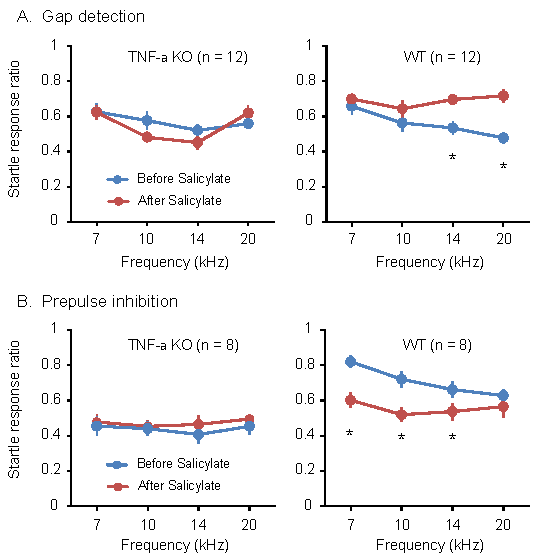
\includegraphics[width=4.5in]{images/C4F2}
	\begin{changemargin}{1in}{1in}
	\footnotesize{Figure 2. Absence of salicylate-induced tinnitus in TNF-\textalpha{} KO mice}
	\end{changemargin}
\end{figure}


\subsection{Cortical infusion of recombinant TNF-\textalpha{} results in tinnitus}

To test whether TNF-\textalpha{} is sufficient to cause tinnitus symptoms, we infused mouse recombinant TNF-\textalpha{} into the right hemisphere auditory cortex of normal-hearing WT and TNF-\textalpha{} KO mice. Control WT and KO mice were infused with carrier solution containing artificial cerebrospinal fluid and mouse albumin. Gap detection and PPI performance was examined in three daily sessions prior to the injection and only the third session was used as the baseline performance. Mice were tested again after 3 days of post-surgical recovery. Gap detection performance was analyzed with a 4-way ANOVA on genotype (WT vs. KO), treatment (before vs. after infusion), drug (TNF-\textalpha{} vs. albumin) and frequency of the background tone. There were main effects of treatment ($F_{1,152}=8.619$, $p=0.0038$) and drug ($F_{1,152}=4.476$, $p=0.032$). There was also treatment $\times$ drug interaction ($F_{1,152}=5.730$, $p=0.018$), indicating that TNF-\textalpha{} and albumin changed gap detection performance differently. However, the interaction was independent of genotype (treatment $\times$ drug $\times$ genotype interaction, $F_{1,152}=0.007$, $p=0.94$) suggesting that TNF-\textalpha{} infusion had similar effects on both WT and KO mice. Post-hoc t-test indicates that TNF-\textalpha{} significantly impaired gap detection at 20 kHz (WT: $t(12)=4.19$, $p=0.0013$; KO: $t(12)=2.45$, $p=0.035$), but not at other frequencies.

A similar 4-way ANOVA on PPI failed to show significant treatment $\times$ drug interaction ($F_{1,152}=0.391$, $p=0.53$) indicating that TNF-\textalpha{} did not alter PPI performance (Figure 3).

\begin{figure}[h]
	\centering
		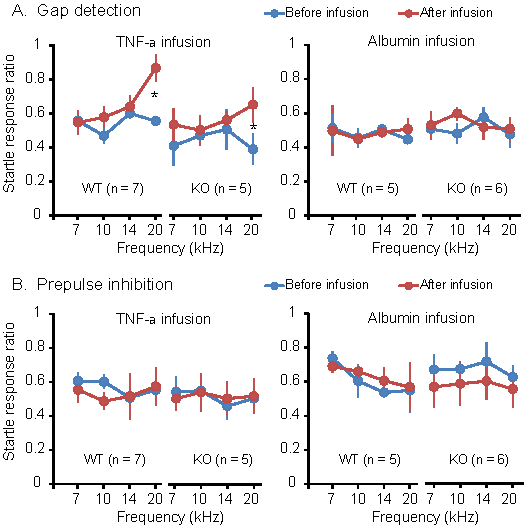
\includegraphics[width=4.5in]{images/C4F3}
	\begin{changemargin}{1in}{1in}
	\footnotesize{Figure 3. TNF-\textalpha{} is sufficient to cause tinnitus. (A) Auditory cortical infusion of mouse recombinant TNF-\textalpha{} results in behavioral signs of tinnitus both WT and TNF-\textalpha{} KO mice, as indicated by impaired gap detection performance. Infusion of mouse albumin did not result in tinnitus. (B) Prepulse inhibition was not altered by infusion of TNF-\textalpha{} or albumin. *$p<0.05$.}
	\end{changemargin}
\end{figure}

\subsection{Hearing loss-induced downregulation of GAD65 expression was reduced in TNF-\textalpha{} KO mice}

GAD65 is an enzyme responsible for synthesizing GABA in the pre-synaptic terminal in response to sustained activation (\cite{Tian1999, Iwai2003}). Hearing loss-induced tinnitus leads to reduced inhibition and lower protein levels of GAD65 in auditory cortex (\cite{Yang2011a}). TNF-\textalpha{} has previously been shown to be important for homeostatic regulation of inhibitory synaptic transmission (\cite{Pribiag2013}), and given the absence of tinnitus in TNF-\textalpha{} KO mice, we hypothesized that they would show altered modulation of inhibition following hearing lesion. NIHL resulted in a $39.9\pm5.1\%$ ($n = 5$) reduction in GAD65 mRNA levels in wildtype mice, but a significantly smaller reduction in TNF-\textalpha{} knockout mice ($17.7\pm4.9\%$; $n=5$; WT versus KO, $p<0.01$), consistent with a role of reduced inhibition in tinnitus etiology (\cite{Yang2011a}).

\begin{figure}[h]
	\centering
		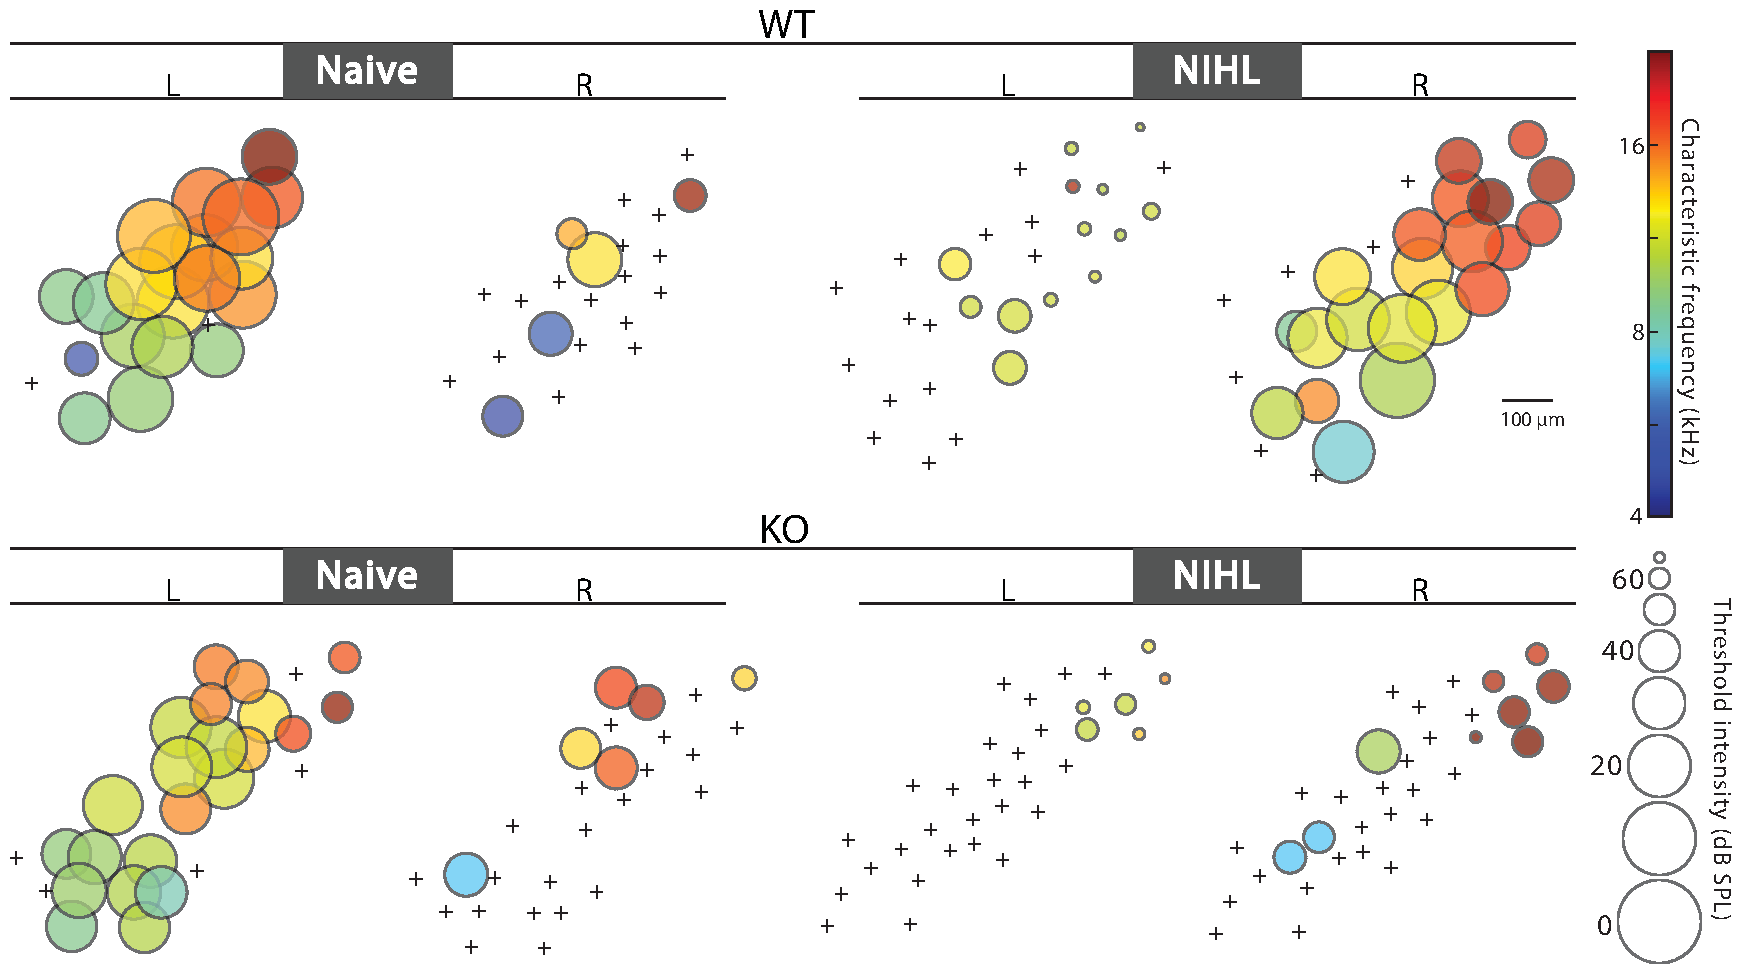
\includegraphics[width=3.25in]{images/C4F4}
	\begin{changemargin}{1in}{1in}
	\footnotesize{Figure 4. TNF-\textalpha{} KO mice experience a smaller GAD65 mRNA reduction following NIHL than WT mice. * indicates a statistically significant difference.}
	\end{changemargin}
\end{figure}

\subsection{Plasticity of ipsilateral inputs following contralateral hearing lesion is impaired in TNF-\textalpha{} KO mice}

To examine the electrophysiological changes in primary auditory cortex following unilateral NIHL, we independently stimulated the lesioned and intact ear while recording multi-unit activity from auditory cortex contralateral to the lesioned ear. Na\"ive WT and KO animals displayed strong, tonotopically-organized RFs in response to contralateral stimulation (Figure 5). Unilateral NIHL led to a drastic reduction in the proportion of units responsive to the lesioned ear in both genotypes, however only in WT mice did NIHL result in a significant increase in the proportion of units responsive to the spared ear in ipsilateral cortex (Na\"ive vs NIHL, WT-Left: $p\ll0.001$, KO-Left: $p=0.0011$, WT-Right: $p=0.012$, KO-Right: $p=0.999$, Tukey's HSD, Figure 6A). As reported previously (\cite{Yang2013}), evoked firing rates are lower in KO animals (WT-Left-na\"ive vs KO-Left-na\"ive, $p=0.0190$, Tukey's HSD, Figure 6B). Evoked firing rate and RF size showed similar patterns of changes following NIHL, i.e., decreases in both genotypes for contralateral stimulation, and increases only in WT animals for ipsilateral stimulation (Na\"ive vs NIHL, mean evoked firing rate: WT-Left: $p\ll0.001$, KO-Left: $p=0.166$, WT-Right: $p=0.045$, KO-Right: $p=1.00$, Figure 5B; RF size: WT-Left: $p\ll0.001$, KO-Left: $p=0.0170$, WT-Right: $p=0.007$, KO-Right: $p=0.999$, Tukey's HSD; Figure 5B,C). One exception was that in KO animals the decrease in mean firing rate for contralateral stimulation post-NIHL did not reach significance. Spontaneous firing rates decreased following hearing lesion, but the effect was not genotype specific (Na\"ive vs NIHL: $p<0.001$, Genotype$\times$Experience interaction: $p=0.63$, not shown).

\begin{sidewaysfigure}[h]
	\centering
		\includegraphics[width=8in]{images/C4F5}
	\begin{changemargin}{1in}{1in}
	\footnotesize{Figure 5. Example contralateral (L) and ipsilateral (R) maps for WT and KO in na\"ive and NIHL animals. Each circle represents the multi-unit recording from one site, with characteristic frequency and threshold intensity represented by color and radius, respectively. Unresponsive sites are marked by a +. In na\"ive WT and KO animals, contralateral maps in na\"ive animals have low thresholds and few non-responsive sites, while ipsilateral maps have few responsive sites. Contralateral responses are nearly eliminated following NIHL in WT and KO, however only WT animals show strong augmentation of the ipsilateral map.}
	\end{changemargin}
\end{sidewaysfigure}


\begin{sidewaysfigure}[h]
	\centering
		\includegraphics[width=8.25in]{images/C4F6}
	\begin{changemargin}{1in}{1in}
	\footnotesize{Figure 6. Characterization of multi-unit electrophysiological data from primary auditory cortex of WT and KO animals pre- and post-NIHL. * $p<0.05$, ** $p<0.01$, *** $p<0.001$, n.s. not significantly different}
	\end{changemargin}
\end{sidewaysfigure}

\section{Discussion}

The precise role of TNF-\textalpha{} in homeostatic plasticity is not entirely clear. Although \textit{in vivo} studies clearly show its necessity for upregulation of AMPARs in response to activity blockade (\cite{Stellwagen2006}), a follow-up study seem to indicate that it plays a permissive rather than instructive role and that TNF-\textalpha{} interacts with the recent history of stimulation and state of synapses. Specifically, TNF-\textalpha{} application leads to the expected synaptic scaling at control synapses, but application to prescaled synapses leads to reduced quantal amplitudes. Also, blocking TNF-\textalpha{} signalling only alters synaptic scaling if performed for 24 hours prior to activity blockade (\cite{Steinmetz2010}). Our data indicates that direct infusion of recombinant TNF-\textalpha{} was sufficient to induce tinnitus in both WT and KO animals. An explanation that is consistent with current understanding of TNF-\textalpha{} operation is that in our na\"ive WT and KO animals, the synapses were in a pre-scaled state, so that TNF-\textalpha{} application led to synaptic upscaling and a tinnitus percept.

We examined the electrophysiological changes that take place in auditory cortex following unilateral noise-induced hearing lesion in WT and KO mice and found that the extensive remapping of ipsilateral input to the deprived contralateral cortex is impaired in the absence of TNF-\textalpha{}. Rapid and extensive ipsilateral remapping following unilateral hearing loss has been observed throughout the auditory pathway (\cite{Mossop2000}). It was long assumed that homeostatic plasticity played a key role in this process, but this is the  first study to provide evidence that TNF-\textalpha{}-related homeostatic plasticity is a critical component. The result has interesting parallels to monocular deprivation-induced remapping of 

% \cite{Kotak2005} increased excitability in auditory cortex following hearing lesion

\printbibliography